\chapter{particular presets} 
\label{sec:presets}
\lstset{style=6502Style}
\lstset{ 
   aboveskip=5pt,
   belowskip=0pt,
}

\begin{definition}[Jeffrey Says]
\setlength{\intextsep}{0pt}%
\setlength{\columnsep}{3pt}%
\begin{wrapfigure}{l}{0.12\textwidth}

\includegraphics[width=\linewidth]{src/callout/psych.png} 
\end{wrapfigure}
\small
SHIFT plus any of the top row of
preset keys: Stores all the parameters for later, instantaneous,
recall by pressing that preset key. Use to store your favourites for
recall instantly without fiddling with all the parameters. 16 presets
available.
\end{definition}

\clearpage                                                                 
\begin{figure}[H]                                                          
  \centering                                                             
  \begin{adjustbox}{width=14cm,center}                                   
  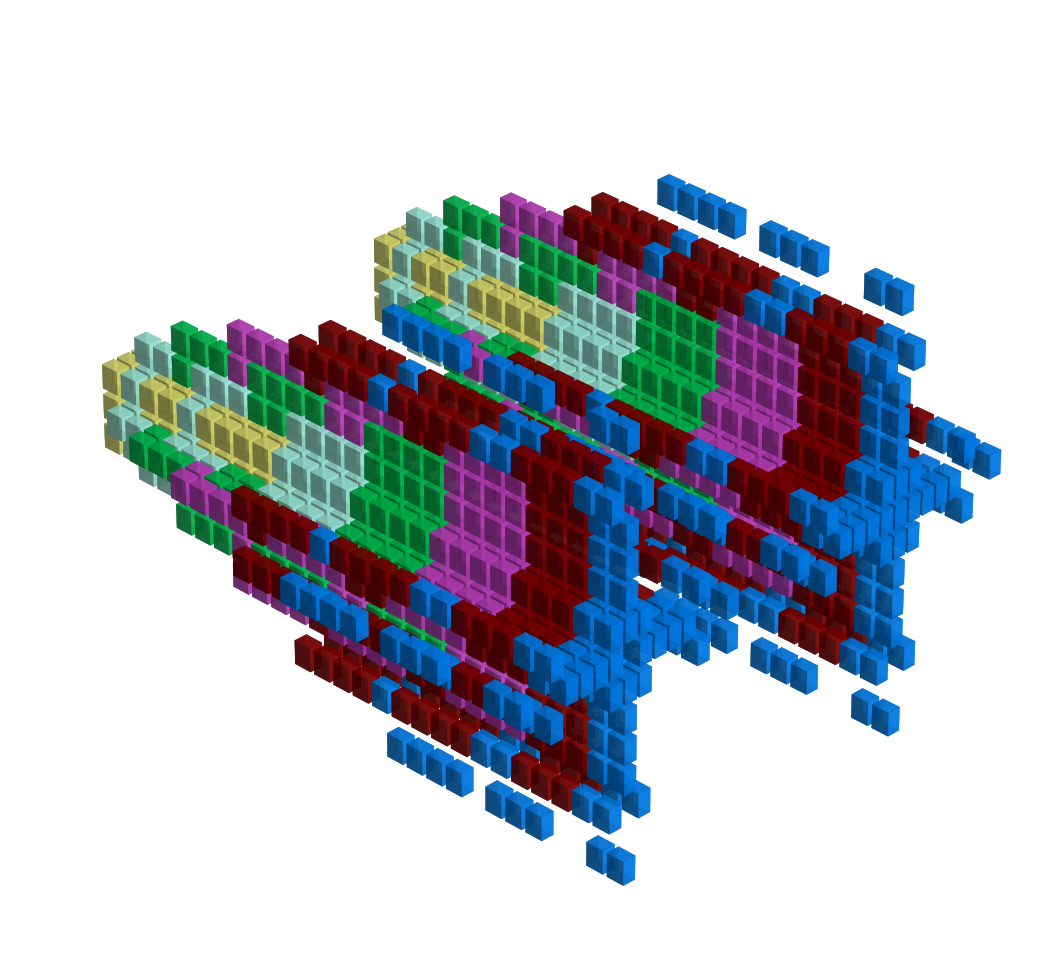
\includegraphics[width=14cm]{src/presets/pattern0-45.png}%           
  \end{adjustbox}                                                        
\caption{Evolution of Preset 0.}                                           
\end{figure}                                                               
\clearpage                                                                 
                                                                           
\begin{lstlisting}[basicstyle=\ttfamily\scriptsize,caption=Data structure for Preset 0.]
;preset0
  ; unusedPresetByte: Unused Byte
  .BYTE $00
  ; smoothingDelay: 'Because of the time taken to draw larger patterns speed
  ; increase/decrease is not linear. You can adjust the 'compensating delay'
  ; which often smooths out jerky patterns. Can be used just for special FX),
  ; though. Suck it and see.'
  .BYTE $0C
  ; cursorSpeed: 'Gives you a slow or fast little cursor, according to setting.'
  .BYTE $02
  ; bufferLength: 'Larger patterns flow more smoothly with a shorter
  ; Buffer Length - not so many positions are retained so less plotting to do.
  ; Small patterns with a long Buffer Length are good for 'steamer' effects.
  ; N.B. Cannot be adjusted whilst patterns are actually onscreen.'
  .BYTE $1F
  ; pulseSpeed: 'Usually if you hold down the button you get a continuous
  ; stream. Setting the Pulse Speed allows you to generate a pulsed stream, as
  ; if you were rapidly pressing and releasing the FIRE button.'
  .BYTE $01
  ; indexForColorBarDisplay: 'The initial index for the color displayed
  ; in the color bar when adjusting the colors for each step.'
  .BYTE $01
  ; lineWidth: 'Sets the width of the lines produced in Line Mode.'
  .BYTE $07
  ; sequencerSpeed: 'Controls the rate at which sequencer feeds in its data. '
  .BYTE $04
  ; pulseWidth: 'Sets the length of the pulses in a pulsed stream output.
  ; Don't worry about what that means - just get in there and mess with it.'
  .BYTE $01
  ; baseLevel: 'Controls how many 'levels' of pattern are plotted.'
  .BYTE $07
  ; presetColorValuesArray: 'Allows you to set the colour for each of the
  ; seven pattern steps. Set up the colour you want, press RETURN, and the
  ; command offers the next colour along, up to no. 7, then ends. Cannot be
  ; adjusted while patterns being generated.'
  .BYTE BLACK,BLUE,RED,PURPLE,GREEN,CYAN,YELLOW,WHITE
  ; trackingActivated: 'Controls whether logic-seeking is used in the
  ; buffer or not. The upshot of this for you is a slightly different feel -
  ; continuous but fragmented when ON, or together-ish bursts when OFF. Try it.'
  .BYTE $00
  ; lineModeActivated: 'A bit like drawing with the Aurora Borealis'
  .BYTE $00
  ; presetIndex: 'This calls in one of the 16 presets, stored Lightsynth
  ; parameters which give different effects. Try them all out io see some uf
  ; the multitude of effects which you cai achieve using the system. Some are
  ; fast, some slow, some pulse, others swirl. Play with them all, try them to
  ; different music.'
  .BYTE $00
  ; currentPatternElement: 'Initial pattern used by this preset.'
  .BYTE $00
  ; currentSymmetrySetting: 'Current symmetry setting.'
  ; Possible values are 0 - 4:
  ; 'NO SYMMETRY     '
  ; 'Y-AXIS SYMMETRY '
  ; 'X-Y SYMMETRY    '
  ; 'X-AXIS SYMMETRY '
  ; 'QUAD SYMMETRY   '
  .BYTE $01
  ; Unused Data.
  .BYTE $FF,$00,$FF,$FF,$00,$FF,$00,$FF,$00
\end{lstlisting}

\clearpage
\textbf{Lines 1189-1231. \icode{\textbf{presetValueArray}}} 
\begin{lstlisting}
; This is where the presets get loaded to. It represents
; the data structure for the presets.
; currentVariableMode is an index into this data structure
; when the user adjusts settings.
presetValueArray
unusedPresetByte        .BYTE $00
smoothingDelay          .BYTE $0C
cursorSpeed             .BYTE $02
bufferLength            .BYTE $1F
pulseSpeed              .BYTE $01
indexForColorBarDisplay .BYTE $01
lineWidth               .BYTE $07
sequencerSpeed          .BYTE $04
pulseWidth              .BYTE $01
baseLevel               .BYTE $07
presetColorValuesArray  .BYTE BLACK,BLUE,RED,PURPLE,GREEN,CYAN,YELLOW,WHITE
trackingActivated       .BYTE $FF
lineModeActivated       .BYTE $00
patternIndex            .BYTE $05
\end{lstlisting}
\textbf{Lines 1189-1231. \icode{\textbf{LoadSelectedPresetSequence}}} 
\begin{lstlisting}
;-----------------------------------------------------
; LoadSelectedPresetSequence
;------------------------------------------------------
LoadSelectedPresetSequence    
        LDA #$FF
        STA currentModeActive

        ; Copy the value from the preset sequence into 
        ; current storage.
        LDY #COLOR_BAR_CURRENT
b16E1   LDA (presetSequenceDataLoPtr),Y
        STA presetValueArray,Y
        INY 
        CPY #$15
        BNE b16E1

        LDA (presetSequenceDataLoPtr),Y
        STA currentPatternElement
        INY 
        LDA (presetSequenceDataLoPtr),Y
        STA currentSymmetrySetting
        JMP WriteLastLineBufferAndReturn
        ; Returns
\end{lstlisting}
\clearpage

\textbf{Lines 1189-1231. \icode{\textbf{presetValueArray}}:} 
text
\textbf{Lines 1189-1231. \icode{\textbf{LoadSelectedPresetSequence}}:} 
\clearpage

\begin{minipage}[b]{0.48\linewidth}
\begin{figure}[H]                                                          
  \centering                                                             
  \begin{adjustbox}{width=7cm,center}                                   
  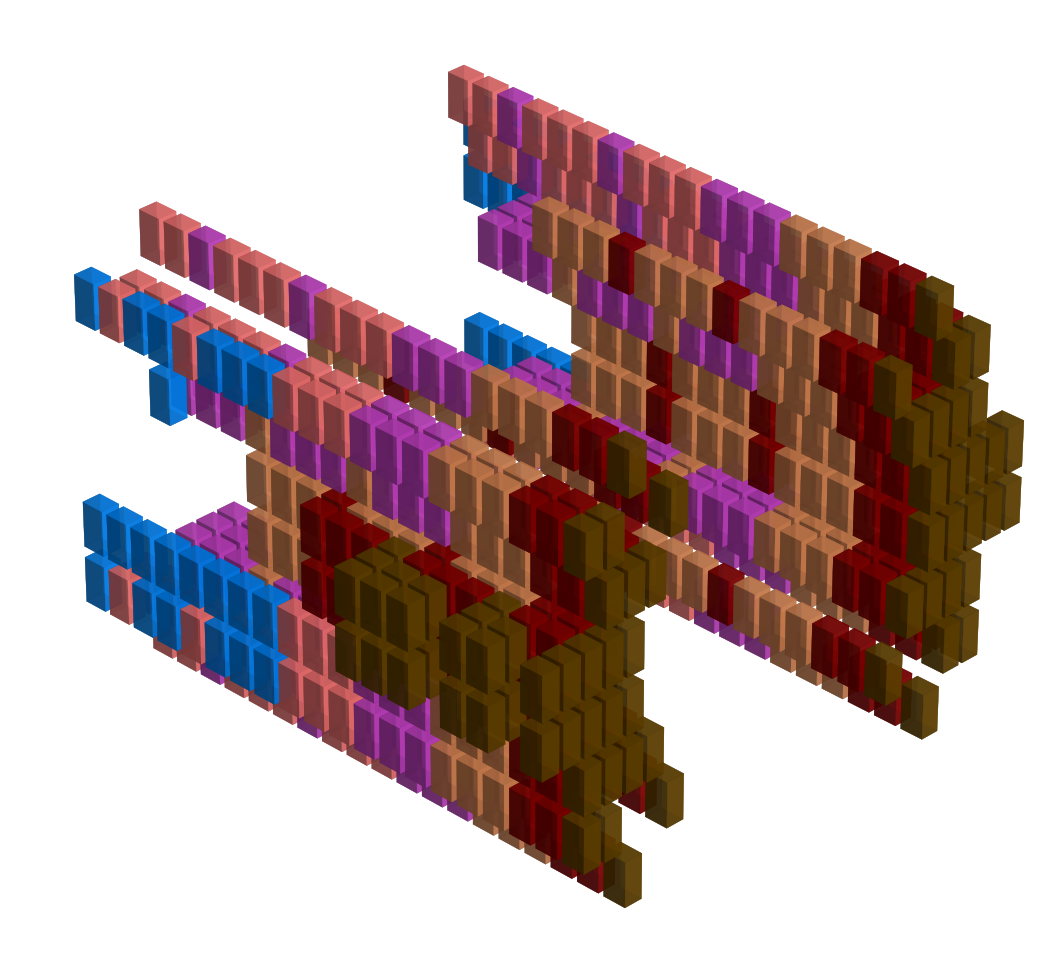
\includegraphics[width=7cm]{src/presets/pattern1-45.png}%           
  \end{adjustbox}                                                        
\caption{Evolution of Preset 1.}                                           
\end{figure}                                                               
\end{minipage}
\hspace{0.1cm}
\begin{minipage}[b]{0.48\linewidth}                            
                                                                           
\begin{lstlisting}[basicstyle=\ttfamily\scriptsize,caption=Data structure for Preset 1.]
preset1
  .BYTE $00 ; unusedPresetByte
  .BYTE $0C ; smoothingDelay
  .BYTE $02 ; cursorSpeed
  .BYTE $28 ; bufferLength
  .BYTE $01 ; pulseSpeed
  .BYTE $0E ; indexForColorBarDisplay
  .BYTE $07 ; lineWidth
  .BYTE $08 ; sequencerSpeed
  .BYTE $01 ; pulseWidth
  .BYTE $07 ; baseLevel
  ; presetColorValuesArray: 
  .BYTE BLACK,BROWN,RED,ORANGE,PURPLE,LTRED,BLUE,LTBLUE
  .BYTE $FF ; trackingActivated
  .BYTE $00 ; lineModeActivated
  .BYTE $01 ; presetIndex
  .BYTE $01 ; currentPatternElement
  .BYTE $04 ; currentSymmetrySetting
\end{lstlisting}
\end{minipage}
\begin{minipage}[b]{0.48\linewidth}

\begin{figure}[H]                                                          
  \centering                                                             
  \begin{adjustbox}{width=7cm,center}                                   
  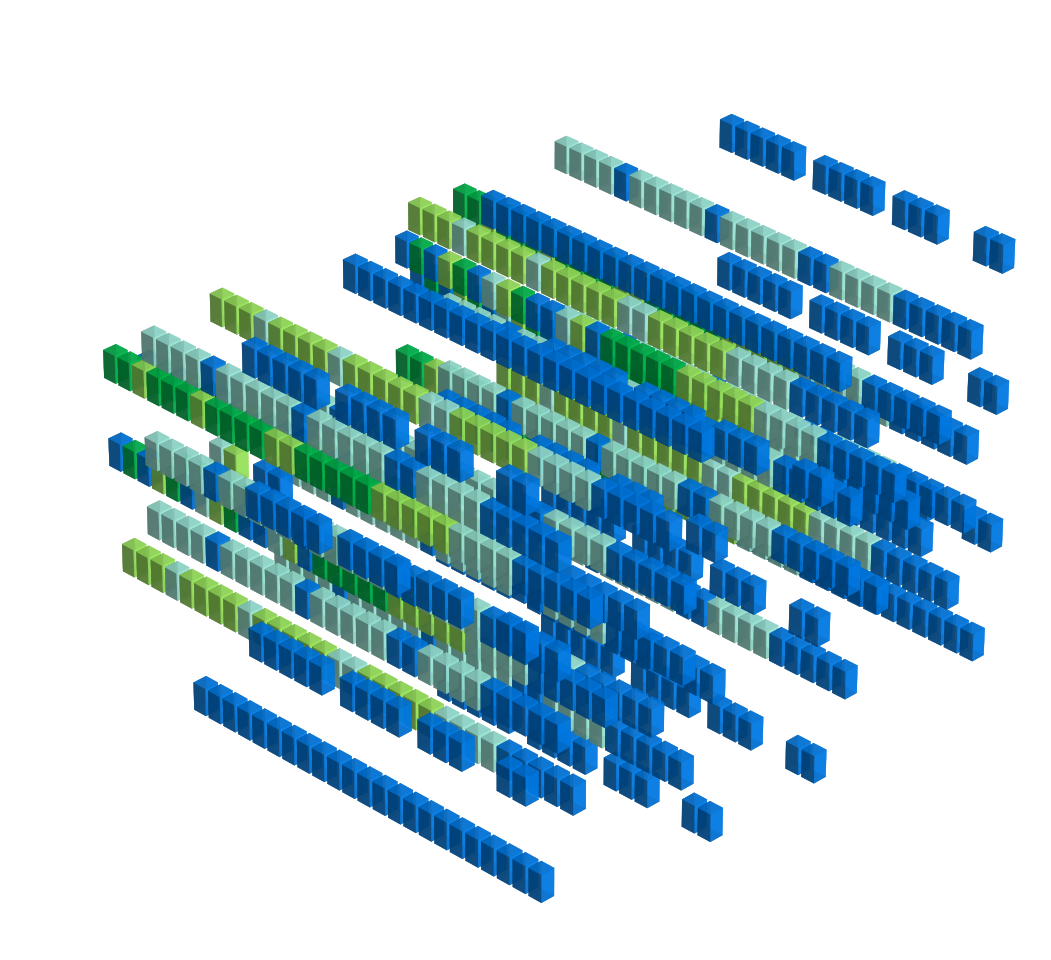
\includegraphics[width=7cm]{src/presets/pattern2-45.png}%           
  \end{adjustbox}                                                        
\caption{Evolution of Preset 2.}                                           
\end{figure}                                                               
\end{minipage}
\hspace{0.1cm}
\begin{minipage}[b]{0.48\linewidth}                            
                                                                           
\begin{lstlisting}[basicstyle=\ttfamily\scriptsize,caption=Data structure for Preset 2.]
preset2
  .BYTE $00 ; unusedPresetByte
  .BYTE $0B ; smoothingDelay
  .BYTE $02 ; cursorSpeed
  .BYTE $28 ; bufferLength
  .BYTE $01 ; pulseSpeed
  .BYTE $01 ; indexForColorBarDisplay
  .BYTE $07 ; lineWidth
  .BYTE $0B ; sequencerSpeed
  .BYTE $01 ; pulseWidth
  .BYTE $07 ; baseLevel
  ; presetColorValuesArray: 
  .BYTE BLACK,BLUE,LTBLUE,CYAN,LTGREEN,GREEN,LTBLUE,BLUE
  .BYTE $FF ; trackingActivated
  .BYTE $00 ; lineModeActivated
  .BYTE $05 ; presetIndex
  .BYTE $05 ; currentPatternElement
  .BYTE $01 ; currentSymmetrySetting
\end{lstlisting}
\end{minipage}


\clearpage
\begin{minipage}[b]{0.48\linewidth}

\begin{figure}[H]                                                          
  \centering                                                             
  \begin{adjustbox}{width=7cm,center}                                   
  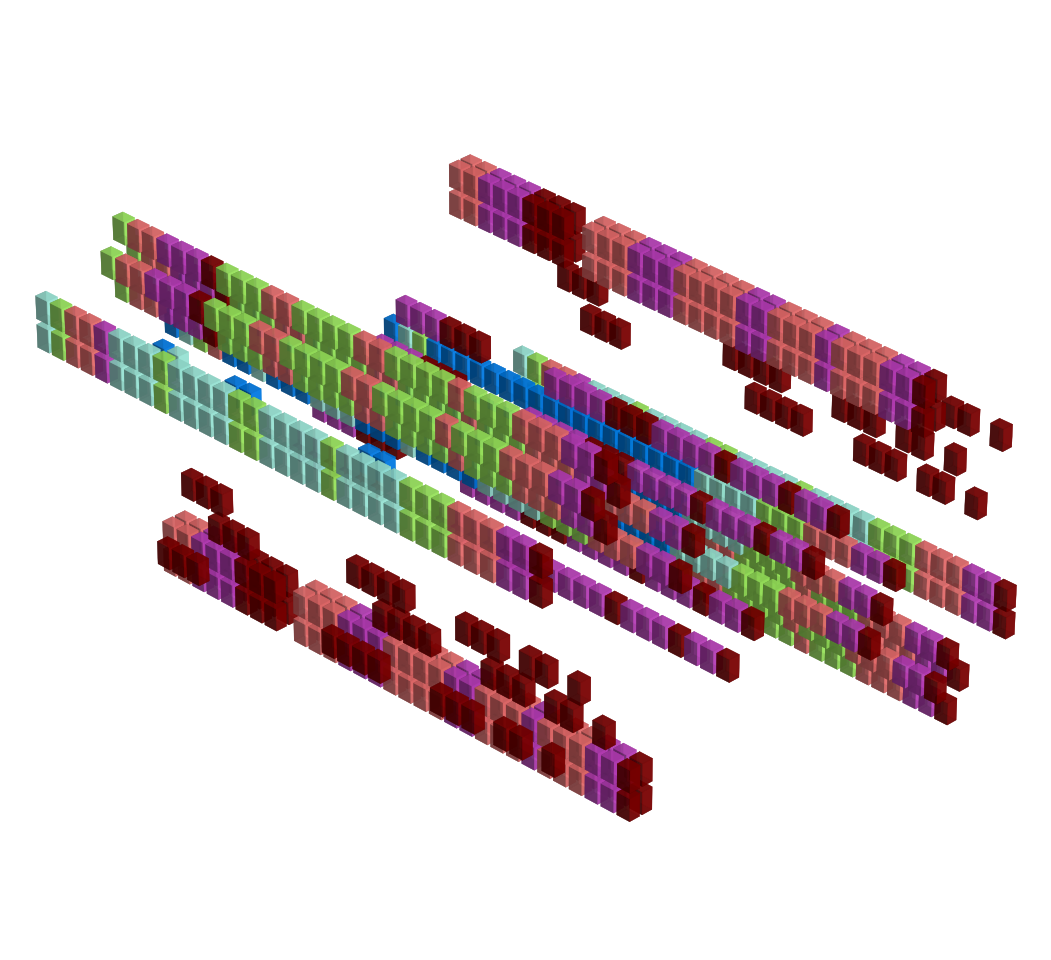
\includegraphics[width=7cm]{src/presets/pattern3-45.png}%           
  \end{adjustbox}                                                        
\caption{Evolution of Preset 3.}                                           
\end{figure}                                                               
\end{minipage}
\hspace{0.1cm}
\begin{minipage}[b]{0.48\linewidth}                            
                                                                           
\begin{lstlisting}[basicstyle=\ttfamily\scriptsize,caption=Data structure for Preset 3.]
preset3
  .BYTE $00 ; unusedPresetByte
  .BYTE $04 ; smoothingDelay
  .BYTE $02 ; cursorSpeed
  .BYTE $26 ; bufferLength
  .BYTE $01 ; pulseSpeed
  .BYTE $01 ; indexForColorBarDisplay
  .BYTE $07 ; lineWidth
  .BYTE $0A ; sequencerSpeed
  .BYTE $01 ; pulseWidth
  .BYTE $07 ; baseLevel
  ; presetColorValuesArray: 
  .BYTE BLACK,RED,PURPLE,LTRED,LTGREEN,CYAN,LTBLUE,BLUE
  .BYTE $00 ; trackingActivated
  .BYTE $00 ; lineModeActivated
  .BYTE $0E ; presetIndex
  .BYTE $0E ; currentPatternElement
  .BYTE $02 ; currentSymmetrySetting
\end{lstlisting}

\end{minipage}
\vspace*{-0.7cm}
\begin{minipage}[b]{0.48\linewidth}
\begin{figure}[H]                                                          
  \centering                                                             
  \begin{adjustbox}{width=7cm,center}                                   
  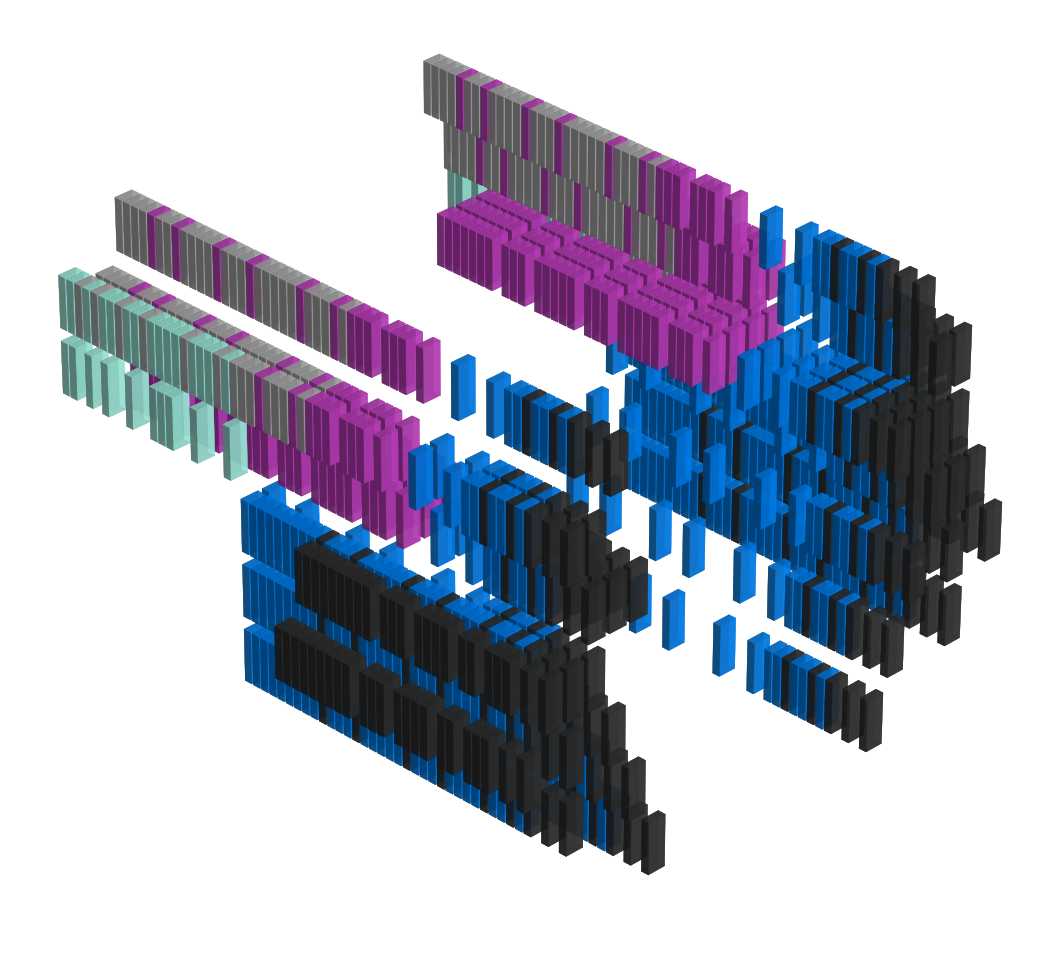
\includegraphics[width=7cm]{src/presets/pattern4-45.png}%           
  \end{adjustbox}                                                        
\caption{Evolution of Preset 4.}                                           
\end{figure}                                                               
\end{minipage}
\hspace{0.1cm}
\begin{minipage}[b]{0.48\linewidth}                            
                                                                           
\begin{lstlisting}[basicstyle=\ttfamily\scriptsize,caption=Data structure for Preset 4.]
preset4
  .BYTE $00 ; unusedPresetByte
  .BYTE $0C ; smoothingDelay
  .BYTE $01 ; cursorSpeed
  .BYTE $2B ; bufferLength
  .BYTE $01 ; pulseSpeed
  .BYTE $07 ; indexForColorBarDisplay
  .BYTE $07 ; lineWidth
  .BYTE $08 ; sequencerSpeed
  .BYTE $01 ; pulseWidth
  .BYTE $07 ; baseLevel
  ; presetColorValuesArray: 
  .BYTE BLACK,GRAY1,BLUE,GRAY2,PURPLE,GRAY3,CYAN,WHITE
  .BYTE $00 ; trackingActivated
  .BYTE $00 ; lineModeActivated
  .BYTE $01 ; presetIndex
  .BYTE $01 ; currentPatternElement
  .BYTE $01 ; currentSymmetrySetting
\end{lstlisting}
\end{minipage}
\clearpage

\clearpage
\textbf{Lines 1189-1231. \icode{\textbf{presetKeyCodes}}} 
\begin{lstlisting}
presetKeyCodes
        .BYTE KEY_LEFT,KEY_1,KEY_2,KEY_3,KEY_4,KEY_5,KEY_6,KEY_7
        .BYTE KEY_8,KEY_9,KEY_0,KEY_PLUS,KEY_MINUS,KEY_POUND
        .BYTE KEY_CLR_HOME,KEY_INST_DEL
\end{lstlisting}
\textbf{Lines 1189-1231. \icode{\textbf{CheckKeyboardInput}}} 
\begin{lstlisting}
;-------------------------------------------------------
; CheckKeyboardInput
;-------------------------------------------------------
CheckKeyboardInput   
        ...
        ; Check if one of the presets has been selected.
CheckIfPresetKeysPressed   
        LDX #$00
presetKeyLoop   
        CMP presetKeyCodes,X
        BEQ UpdateDisplayedPreset
        INX 
        CPX #$10
        BNE presetKeyLoop

        JMP MaybeWPressed

UpdateDisplayedPreset   
        JMP DisplayPresetMessage
\end{lstlisting}

\clearpage

\textbf{Lines 1189-1231. \icode{\textbf{CheckIfPresetKeysPressed}}:} 
\clearpage
\begin{minipage}[b]{0.48\linewidth}

\begin{figure}[H]                                                          
  \centering                                                             
  \begin{adjustbox}{width=7cm,center}                                   
  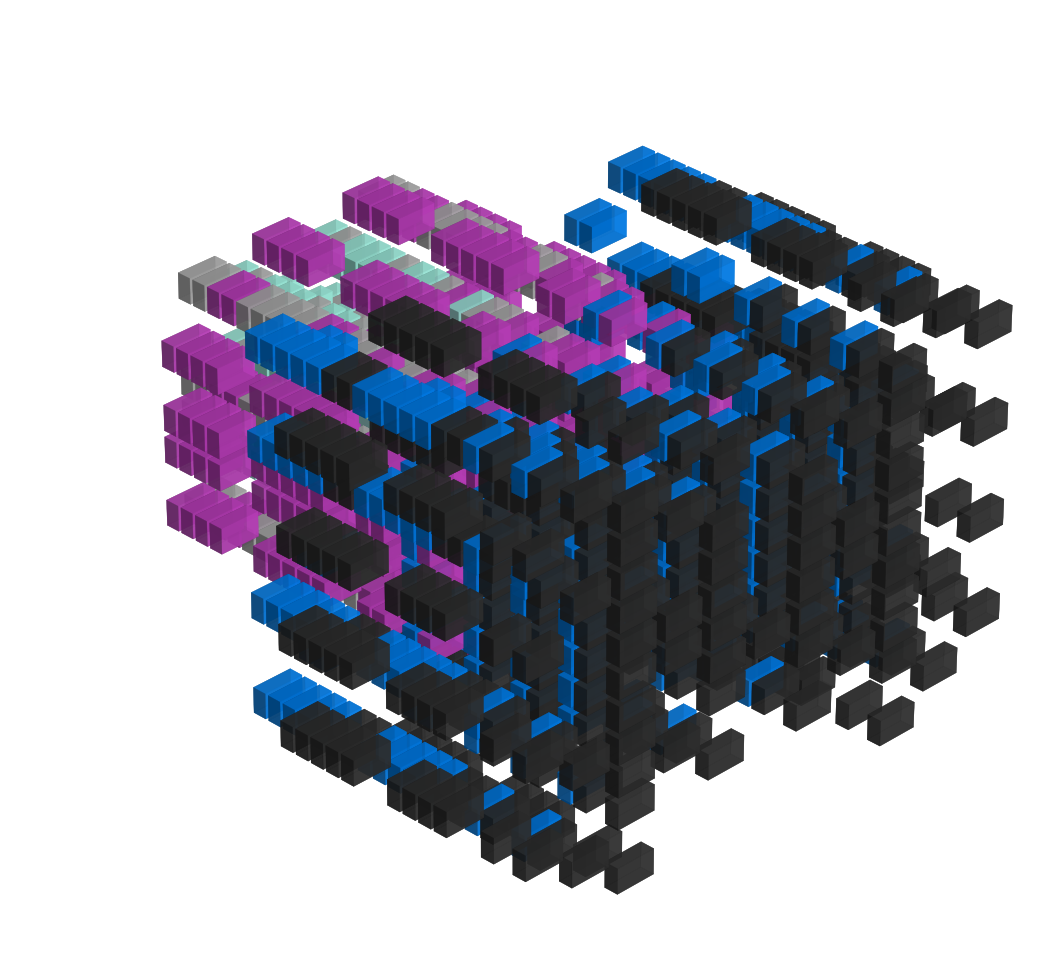
\includegraphics[width=7cm]{src/presets/pattern5-45.png}%           
  \end{adjustbox}                                                        
\caption{Evolution of Preset 5.}                                           
\end{figure}                                                               
\end{minipage}
\hspace{0.1cm}
\begin{minipage}[b]{0.48\linewidth}                                       
                                                                           
\begin{lstlisting}[basicstyle=\ttfamily\scriptsize,caption=Data structure for Preset 5.]
preset5
  .BYTE $00 ; unusedPresetByte
  .BYTE $0C ; smoothingDelay
  .BYTE $02 ; cursorSpeed
  .BYTE $2B ; bufferLength
  .BYTE $01 ; pulseSpeed
  .BYTE $07 ; indexForColorBarDisplay
  .BYTE $07 ; lineWidth
  .BYTE $0C ; sequencerSpeed
  .BYTE $01 ; pulseWidth
  .BYTE $07 ; baseLevel
  ; presetColorValuesArray: 
  .BYTE BLACK,GRAY1,BLUE,GRAY2,PURPLE,GRAY3,CYAN,WHITE
  .BYTE $00 ; trackingActivated
  .BYTE $00 ; lineModeActivated
  .BYTE $06 ; presetIndex
  .BYTE $06 ; currentPatternElement
  .BYTE $03 ; currentSymmetrySetting
\end{lstlisting}
\end{minipage}

\vspace*{-0.7cm}
\begin{minipage}[b]{0.48\linewidth}


                                                                 
\begin{figure}[H]                                                          
  \centering                                                             
  \begin{adjustbox}{width=7cm,center}                                   
  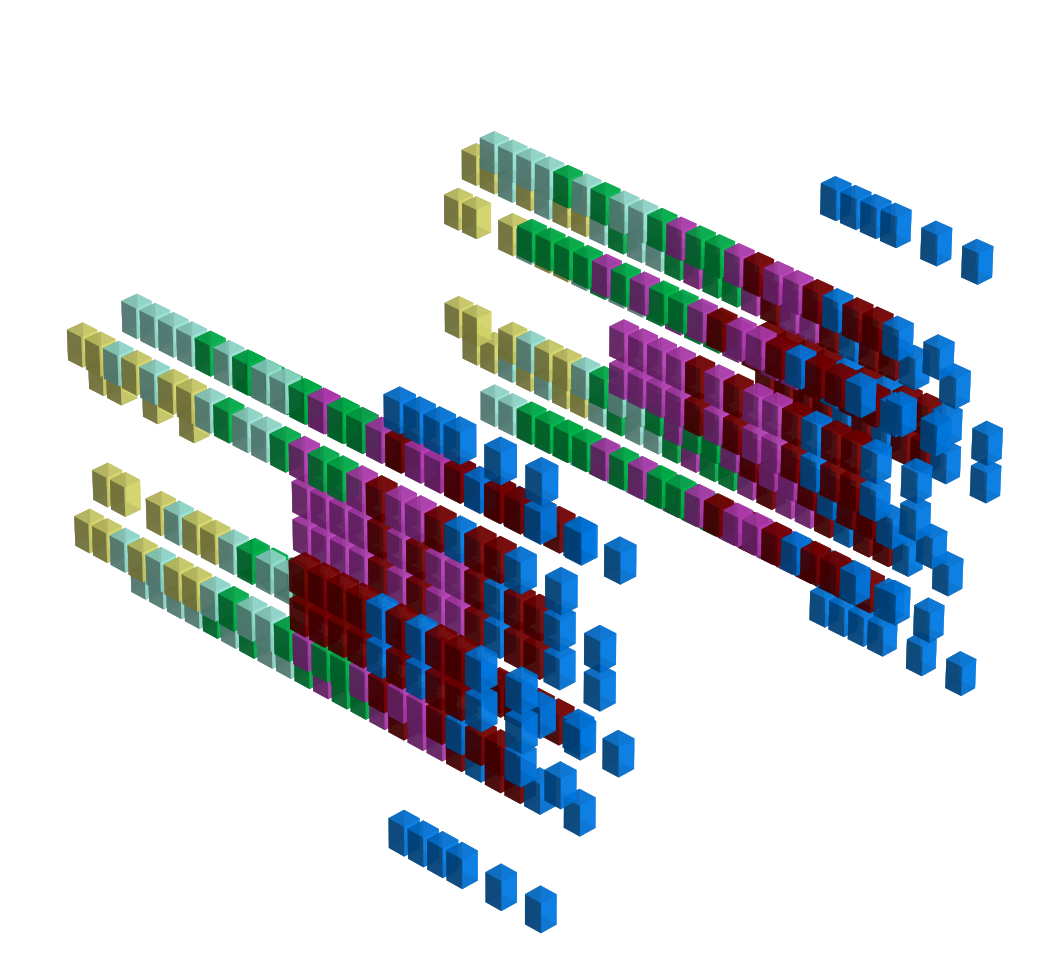
\includegraphics[width=7cm]{src/presets/pattern6-45.png}%           
  \end{adjustbox}                                                        
\caption{Evolution of Preset 6.}                                           
\end{figure}                                                               
                                                                 
                                                                           
\end{minipage}
\hspace{0.1cm}
\begin{minipage}[b]{0.48\linewidth}                                       
\begin{lstlisting}[basicstyle=\ttfamily\scriptsize,caption=Data structure for Preset 6.]
preset6
  .BYTE $00 ; unusedPresetByte
  .BYTE $0F ; smoothingDelay
  .BYTE $02 ; cursorSpeed
  .BYTE $3F ; bufferLength
  .BYTE $01 ; pulseSpeed
  .BYTE $01 ; indexForColorBarDisplay
  .BYTE $07 ; lineWidth
  .BYTE $0F ; sequencerSpeed
  .BYTE $01 ; pulseWidth
  .BYTE $07 ; baseLevel
  ; presetColorValuesArray: 
  .BYTE BLACK,BLUE,RED,PURPLE,GREEN,CYAN,YELLOW,WHITE
  .BYTE $FF ; trackingActivated
  .BYTE $00 ; lineModeActivated
  .BYTE $03 ; presetIndex
  .BYTE $03 ; currentPatternElement
  .BYTE $04 ; currentSymmetrySetting
\end{lstlisting}
\end{minipage}

\clearpage
\begin{minipage}[b]{0.48\linewidth}


                                                                 
\begin{figure}[H]                                                          
  \centering                                                             
  \begin{adjustbox}{width=7cm,center}                                   
  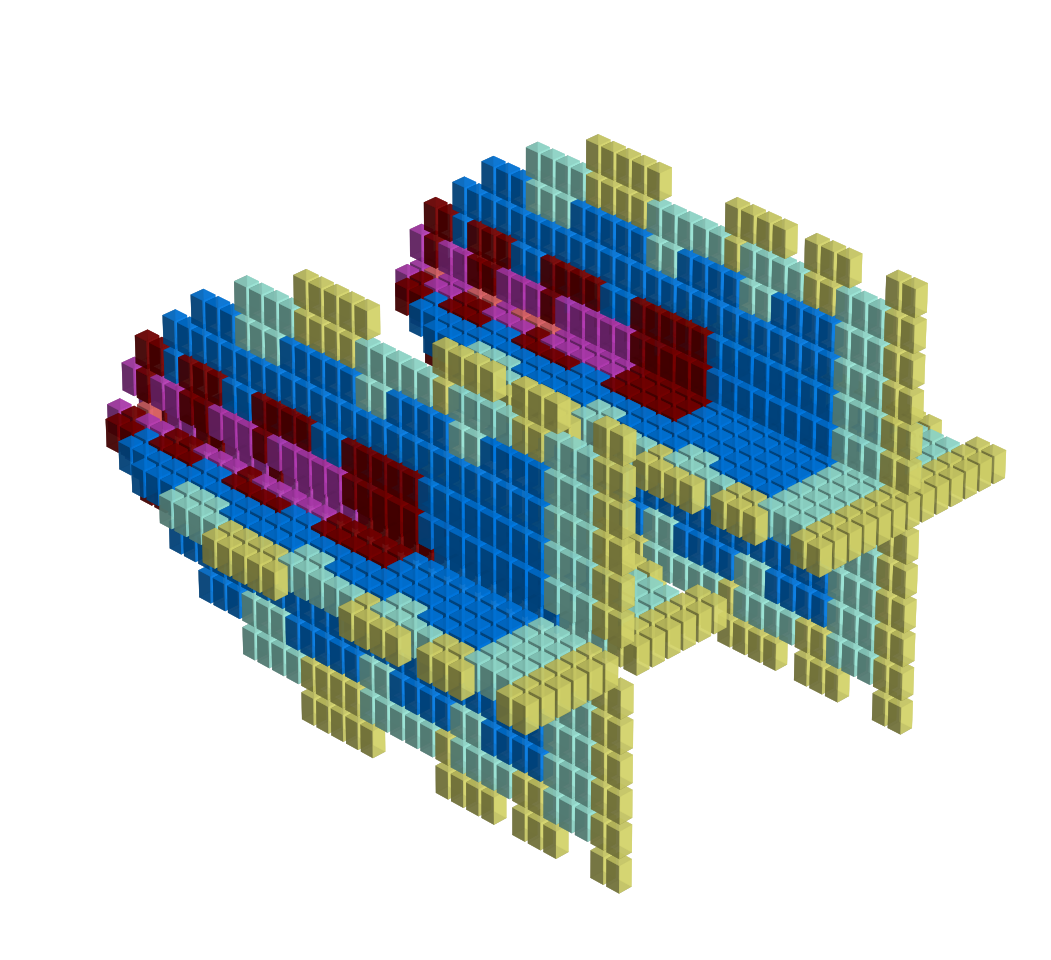
\includegraphics[width=7cm]{src/presets/pattern7-45.png}%           
  \end{adjustbox}                                                        
\caption{Evolution of Preset 7.}                                           
\end{figure}                                                               
                                                                 
                                                                           
\end{minipage}
\hspace{0.1cm}
\begin{minipage}[b]{0.48\linewidth}                                       
\begin{lstlisting}[basicstyle=\ttfamily\scriptsize,caption=Data structure for Preset 7.]
preset7
  .BYTE $00 ; unusedPresetByte
  .BYTE $0B ; smoothingDelay
  .BYTE $01 ; cursorSpeed
  .BYTE $1C ; bufferLength
  .BYTE $02 ; pulseSpeed
  .BYTE $0A ; indexForColorBarDisplay
  .BYTE $07 ; lineWidth
  .BYTE $09 ; sequencerSpeed
  .BYTE $01 ; pulseWidth
  .BYTE $07 ; baseLevel
  ; presetColorValuesArray: 
  .BYTE BLACK,YELLOW,CYAN,LTBLUE,BLUE,RED,PURPLE,LTRED
  .BYTE $00 ; trackingActivated
  .BYTE $00 ; lineModeActivated
  .BYTE $07 ; presetIndex
  .BYTE $07 ; currentPatternElement
  .BYTE $01 ; currentSymmetrySetting
\end{lstlisting}
\end{minipage}

\begin{minipage}[b]{0.48\linewidth}
\begin{figure}[H]                                                          
  \centering                                                             
  \begin{adjustbox}{width=7cm,center}                                   
  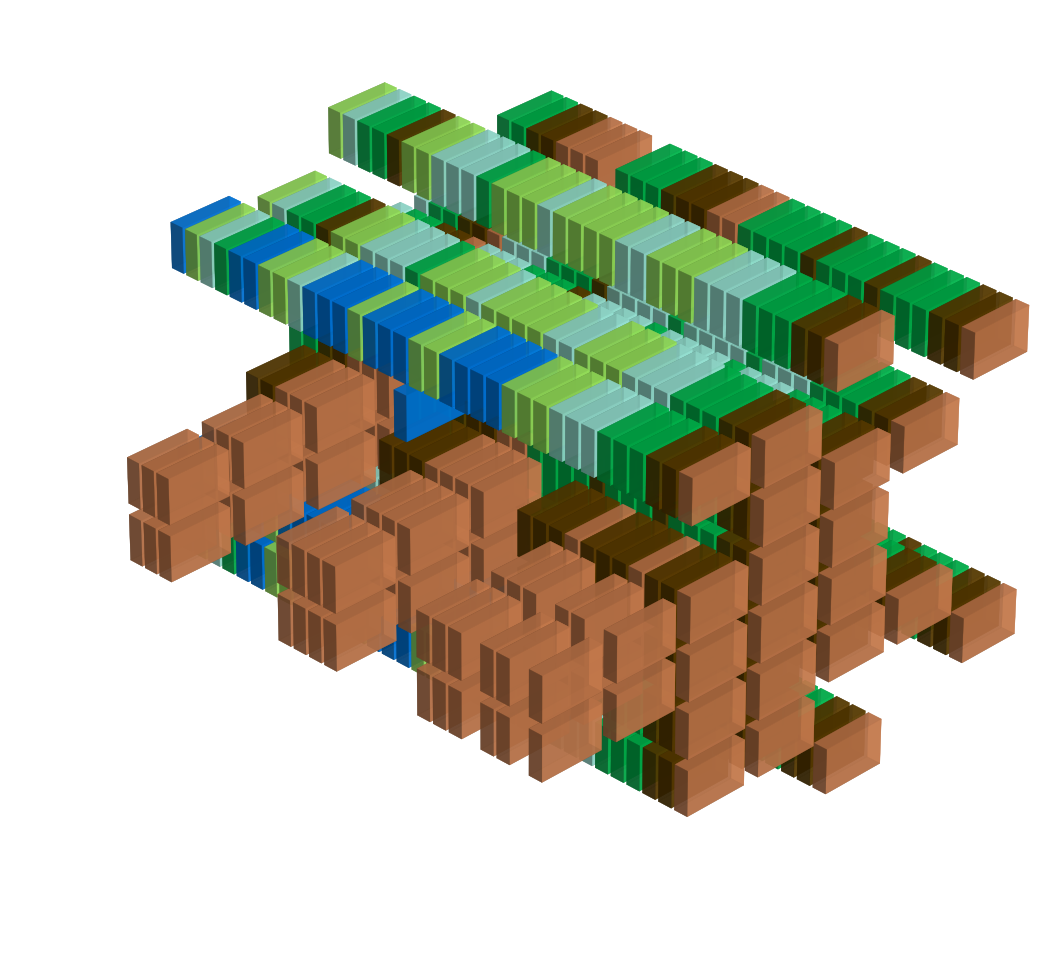
\includegraphics[width=7cm]{src/presets/pattern8-45.png}%           
  \end{adjustbox}                                                        
\caption{Evolution of Preset 8.}                                           
\end{figure}                                                               
                                                                 
                                                                           
\end{minipage}
\hspace{0.1cm}
\begin{minipage}[b]{0.48\linewidth}                                       
\begin{lstlisting}[basicstyle=\ttfamily\scriptsize,caption=Data structure for Preset 8.]
preset8
  .BYTE $00 ; unusedPresetByte
  .BYTE $04 ; smoothingDelay
  .BYTE $01 ; cursorSpeed
  .BYTE $28 ; bufferLength
  .BYTE $02 ; pulseSpeed
  .BYTE $01 ; indexForColorBarDisplay
  .BYTE $07 ; lineWidth
  .BYTE $0A ; sequencerSpeed
  .BYTE $01 ; pulseWidth
  .BYTE $07 ; baseLevel
  ; presetColorValuesArray: 
  .BYTE BLACK,ORANGE,BROWN,GREEN,CYAN,LTGREEN,LTBLUE,BLUE
  .BYTE $FF ; trackingActivated
  .BYTE $00 ; lineModeActivated
  .BYTE $01 ; presetIndex
  .BYTE $01 ; currentPatternElement
  .BYTE $03 ; currentSymmetrySetting
\end{lstlisting}
\end{minipage}


\clearpage
\textbf{Lines 1189-1231. \icode{\textbf{DisplayPresetMessage}}} 
\begin{lstlisting}
;-------------------------------------------------------
; DisplayPresetMessage
;-------------------------------------------------------
DisplayPresetMessage    
        LDA shiftPressed
        AND #$04
        BEQ SelectNewPreset
        JMP EditCustomPattern

SelectNewPreset
        TXA 
        PHA 
        JSR ClearLastLineOfScreen
        LDX #$00
b1613   LDA txtPreset,X
        STA lastLineBufferPtr,X
        INX 
        CPX #$10
        BNE b1613

        PLA 
        PHA 
        TAX 
        BEQ b1638
b1623   INC dataFreeDigitThree
        LDA dataFreeDigitThree
        CMP #$BA
        BNE b1635
        LDA #$30
        STA dataFreeDigitThree
        INC dataFreeDigitTwo
b1635   DEX 
        BNE b1623

b1638   JMP UpdateCurrentActivePreset

WriteLastLineBufferAndReturn    
        JSR WriteLastLineBufferToScreen
        RTS 

.enc "petscii" 
txtPreset
        .TEXT 'PRESET ',$B0,$B0,'      ',$BA
txtPresetActivatedStored
        .TEXT ' ACTIVATED       '
        .TEXT 'DATA STORED    '
.enc "none" 
\end{lstlisting}
\clearpage

\textbf{Lines 1189-1231. \icode{\textbf{DisplayPresetMessage}}:} 
\clearpage
\begin{minipage}[b]{0.48\linewidth}
\begin{figure}[H]                                                          
  \centering                                                             
  \begin{adjustbox}{width=7cm,center}                                   
  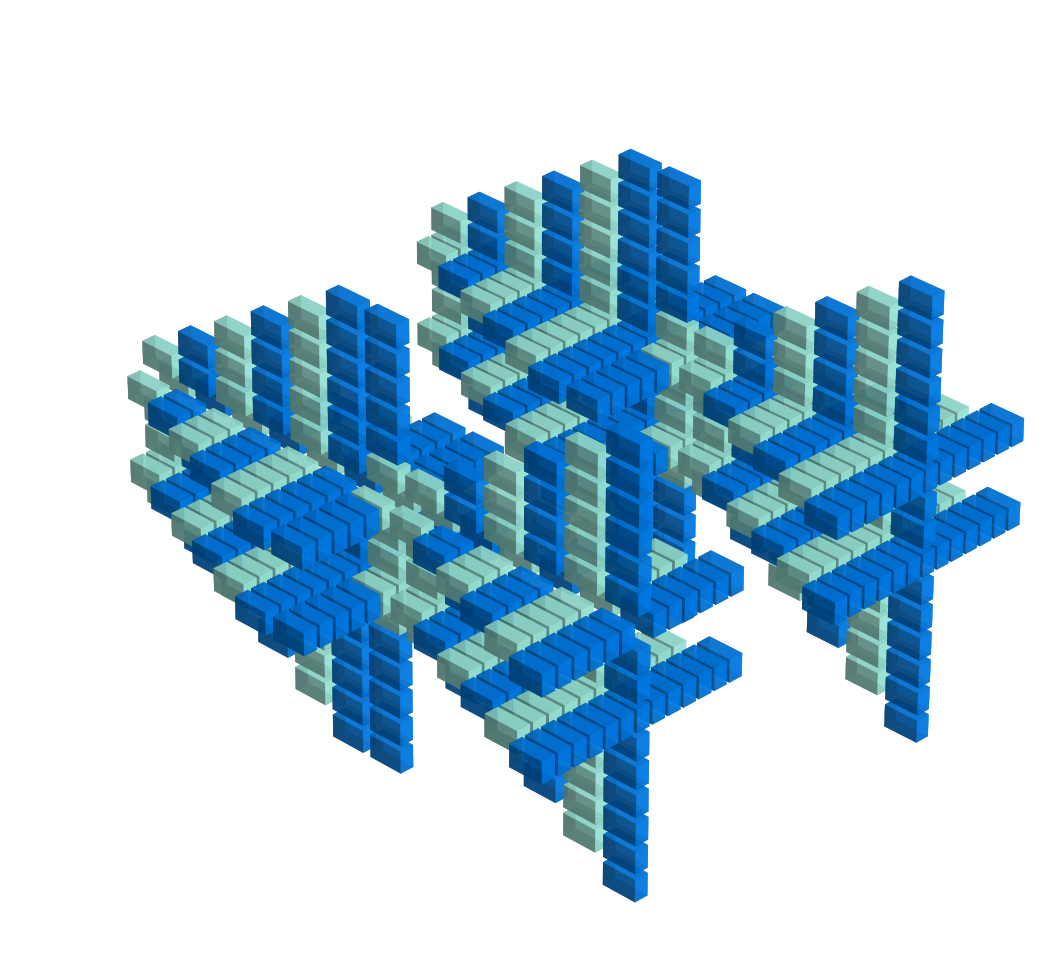
\includegraphics[width=7cm]{src/presets/pattern9-45.png}%           
  \end{adjustbox}                                                        
\caption{Evolution of Preset 9.}                                           
\end{figure}                                                               
\end{minipage}
\hspace{0.1cm}
\begin{minipage}[b]{0.48\linewidth}                                       
\begin{lstlisting}[basicstyle=\ttfamily\scriptsize,caption=Data structure for Preset 9.]
preset9
  .BYTE $00 ; unusedPresetByte
  .BYTE $11 ; smoothingDelay
  .BYTE $01 ; cursorSpeed
  .BYTE $0D ; bufferLength
  .BYTE $07 ; pulseSpeed
  .BYTE $01 ; indexForColorBarDisplay
  .BYTE $07 ; lineWidth
  .BYTE $0C ; sequencerSpeed
  .BYTE $01 ; pulseWidth
  .BYTE $07 ; baseLevel
  ; presetColorValuesArray: 
  .BYTE BLACK,BLUE,CYAN,BLUE,CYAN,BLUE,CYAN,BLUE
  .BYTE $FF ; trackingActivated
  .BYTE $00 ; lineModeActivated
  .BYTE $07 ; presetIndex
  .BYTE $07 ; currentPatternElement
  .BYTE $04 ; currentSymmetrySetting
\end{lstlisting}
\end{minipage}

\vspace*{-0.7cm}
\begin{minipage}[b]{0.48\linewidth}


                                                                 
\begin{figure}[H]                                                          
  \centering                                                             
  \begin{adjustbox}{width=7cm,center}                                   
  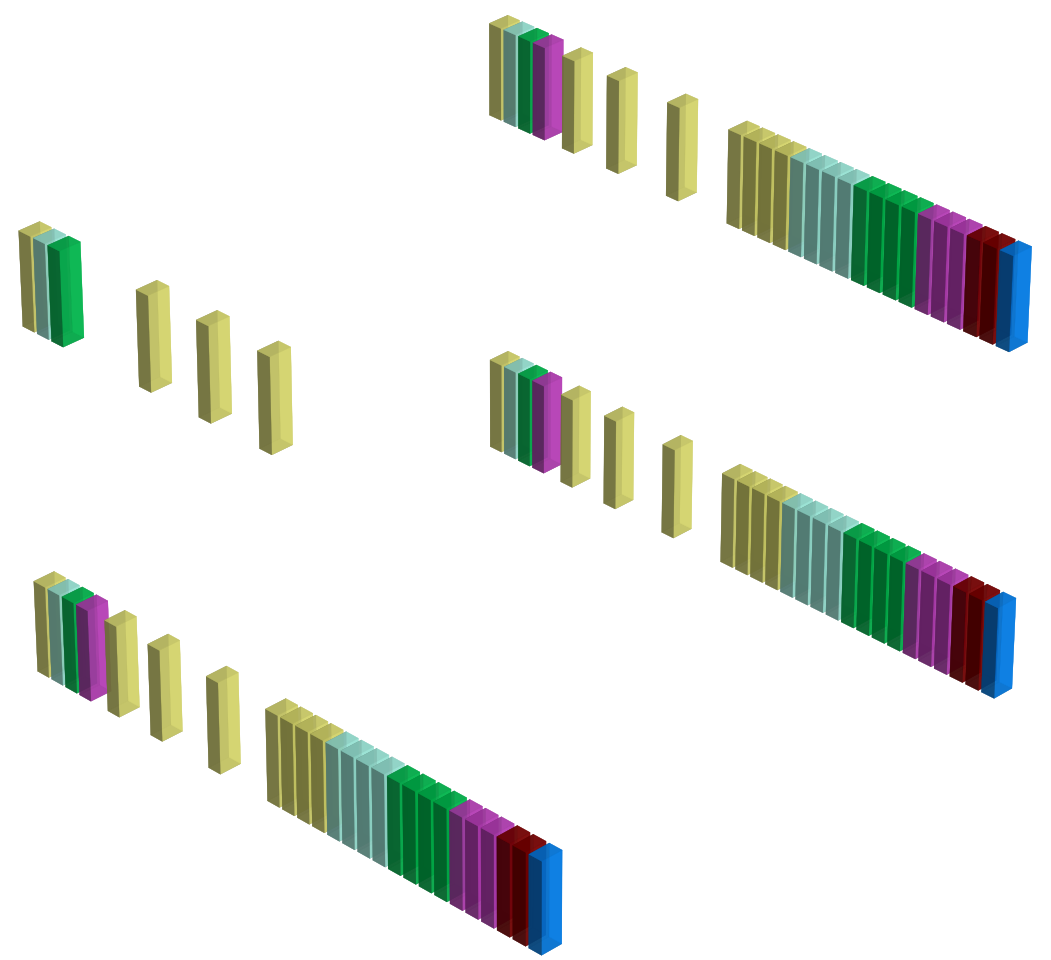
\includegraphics[width=7cm]{src/presets/pattern10-45.png}%           
  \end{adjustbox}                                                        
\caption{Evolution of Preset 10.}                                           
\end{figure}                                                               
                                                                 
                                                                           
\end{minipage}
\hspace{0.1cm}
\begin{minipage}[b]{0.48\linewidth}                                       
\begin{lstlisting}[basicstyle=\ttfamily\scriptsize,caption=Data structure for Preset 10.]
preset10
  .BYTE $00 ; unusedPresetByte
  .BYTE $01 ; smoothingDelay
  .BYTE $02 ; cursorSpeed
  .BYTE $1F ; bufferLength
  .BYTE $02 ; pulseSpeed
  .BYTE $09 ; indexForColorBarDisplay
  .BYTE $04 ; lineWidth
  .BYTE $08 ; sequencerSpeed
  .BYTE $01 ; pulseWidth
  .BYTE $07 ; baseLevel
  ; presetColorValuesArray: 
  .BYTE BLACK,BLUE,RED,RED,PURPLE,LTRED,ORANGE,BROWN
  .BYTE $FF ; trackingActivated
  .BYTE $01 ; lineModeActivated
  .BYTE $00 ; presetIndex
  .BYTE $00 ; currentPatternElement
  .BYTE $04 ; currentSymmetrySetting
\end{lstlisting}
\end{minipage}

\clearpage
\begin{minipage}[b]{0.48\linewidth}
\begin{figure}[H]                                                          
  \centering                                                             
  \begin{adjustbox}{width=7cm,center}                                   
  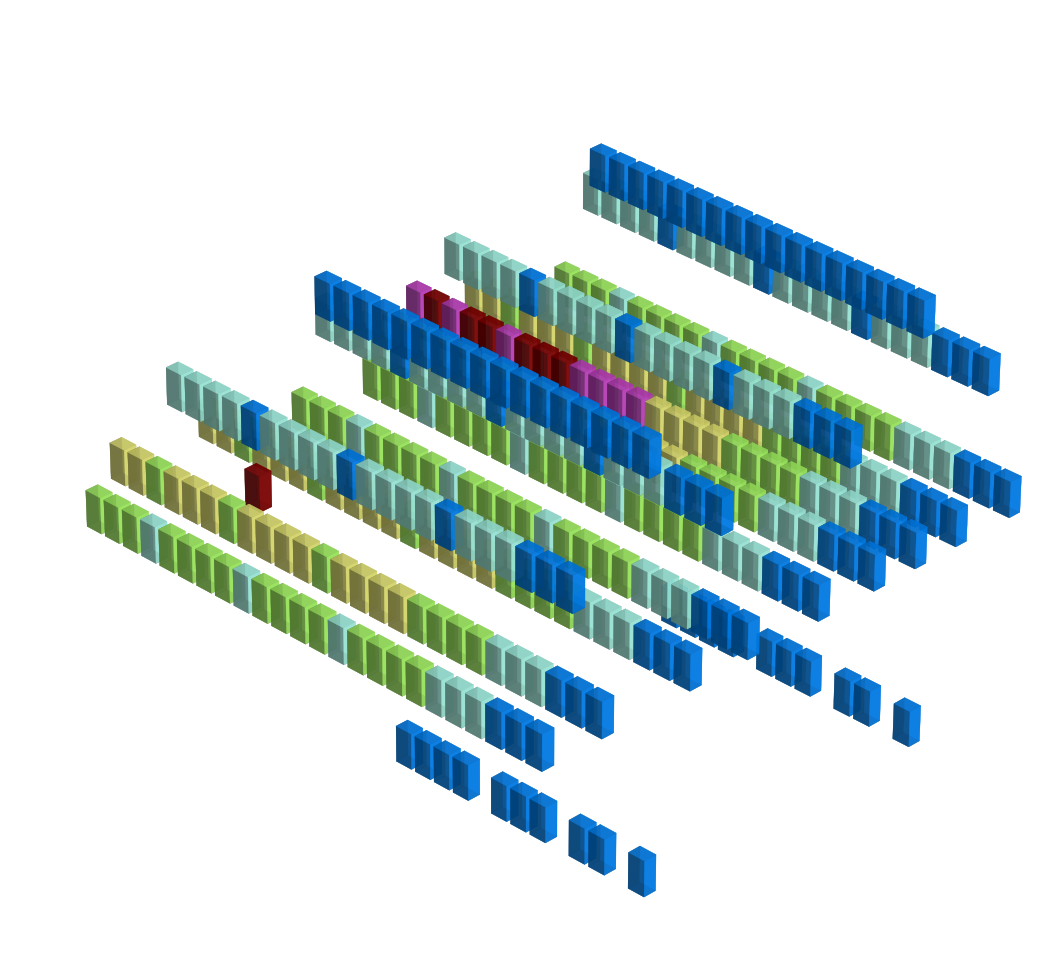
\includegraphics[width=7cm]{src/presets/pattern11-45.png}%           
  \end{adjustbox}                                                        
\caption{Evolution of Preset 11.}                                           
\end{figure}                                                               
                                                                 
                                                                           
\end{minipage}
\hspace{0.1cm}
\begin{minipage}[b]{0.48\linewidth}                                       
\begin{lstlisting}[basicstyle=\ttfamily\scriptsize,caption=Data structure for Preset 11.]
preset11
  .BYTE $00 ; unusedPresetByte
  .BYTE $01 ; smoothingDelay
  .BYTE $01 ; cursorSpeed
  .BYTE $13 ; bufferLength
  .BYTE $06 ; pulseSpeed
  .BYTE $01 ; indexForColorBarDisplay
  .BYTE $07 ; lineWidth
  .BYTE $08 ; sequencerSpeed
  .BYTE $05 ; pulseWidth
  .BYTE $07 ; baseLevel
  ; presetColorValuesArray: 
  .BYTE BLACK,BLUE,RED,PURPLE,GREEN,CYAN,YELLOW,WHITE
  .BYTE $FF ; trackingActivated
  .BYTE $00 ; lineModeActivated
  .BYTE $0F ; presetIndex
  .BYTE $0F ; currentPatternElement
  .BYTE $04 ; currentSymmetrySetting
\end{lstlisting}
\end{minipage}

\vspace*{-0.7cm}
\begin{minipage}[b]{0.48\linewidth}


                                                                 
\begin{figure}[H]                                                          
  \centering                                                             
  \begin{adjustbox}{width=7cm,center}                                   
  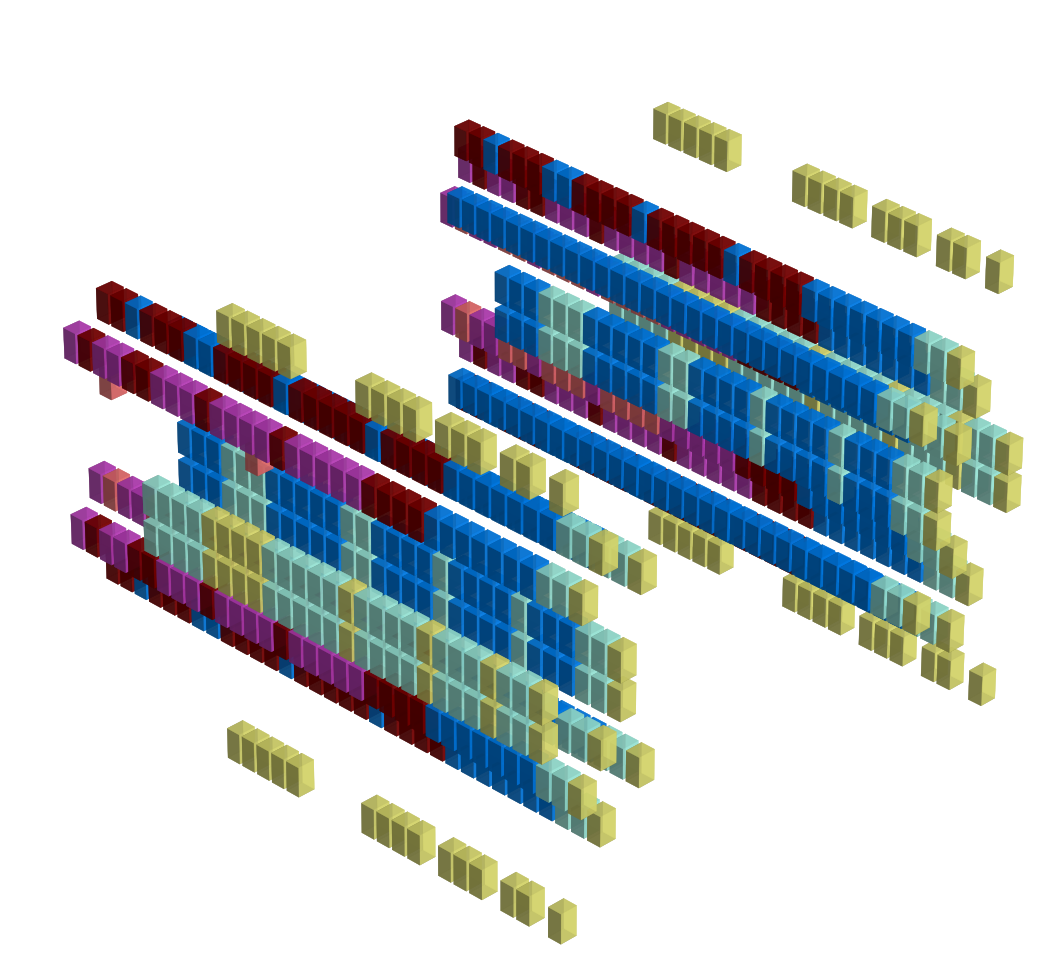
\includegraphics[width=7cm]{src/presets/pattern12-45.png}%           
  \end{adjustbox}                                                        
\caption{Evolution of Preset 12.}                                           
\end{figure}                                                               
                                                                 
                                                                           
\end{minipage}
\hspace{0.1cm}
\begin{minipage}[b]{0.48\linewidth}                                       
\begin{lstlisting}[basicstyle=\ttfamily\scriptsize,caption=Data structure for Preset 12.]
preset12
  .BYTE $00 ; unusedPresetByte
  .BYTE $0C ; smoothingDelay
  .BYTE $02 ; cursorSpeed
  .BYTE $28 ; bufferLength
  .BYTE $01 ; pulseSpeed
  .BYTE $02 ; indexForColorBarDisplay
  .BYTE $07 ; lineWidth
  .BYTE $09 ; sequencerSpeed
  .BYTE $01 ; pulseWidth
  .BYTE $07 ; baseLevel
  ; presetColorValuesArray: 
  .BYTE BLACK,BLUE,LTBLUE,CYAN,LTGREEN,YELLOW,PURPLE,RED
  .BYTE $00 ; trackingActivated
  .BYTE $00 ; lineModeActivated
  .BYTE $0A ; presetIndex
  .BYTE $0A ; currentPatternElement
  .BYTE $01 ; currentSymmetrySetting
\end{lstlisting}
\end{minipage}

\clearpage
\textbf{Lines 1189-1231. \icode{\textbf{UpdateCurrentActivePreset}}} 
\begin{lstlisting}
;-------------------------------------------------------
; UpdateCurrentActivePreset
;-------------------------------------------------------
UpdateCurrentActivePreset    
        LDA shiftPressed
        AND #$01
        ASL 
        ASL 
        ASL 
        ASL 
        TAY 

        LDX #$00
b167C   LDA txtPresetActivatedStored,Y
        STA customPatternValueBufferMessage,X
        INY 
        INX 
        CPX #$10
        BNE b167C

        LDA shiftPressed
        AND #$01
        BNE b1692
        JMP RefreshPresetData

b1692   PLA 
        TAX 
        JSR GetPresetPointersUsingXRegister

        LDY #$00
        LDX #$00
b169B   LDA presetValueArray,X
        STA (presetSequenceDataLoPtr),Y
        INY 
        INX 
        CPX #$15
        BNE b169B

        LDA currentPatternElement
        STA (presetSequenceDataLoPtr),Y
        INY 
        LDA currentSymmetrySetting
        STA (presetSequenceDataLoPtr),Y
        JMP WriteLastLineBufferAndReturn
\end{lstlisting}
\clearpage

\textbf{Lines 1189-1231. \icode{\textbf{UpdateCurrentActivePreset}}:} 
\clearpage
\vspace*{-0.5cm}
\begin{minipage}[b]{0.48\linewidth}


                                                                 
\begin{figure}[H]                                                          
  \centering                                                             
  \begin{adjustbox}{width=7cm,center}                                   
  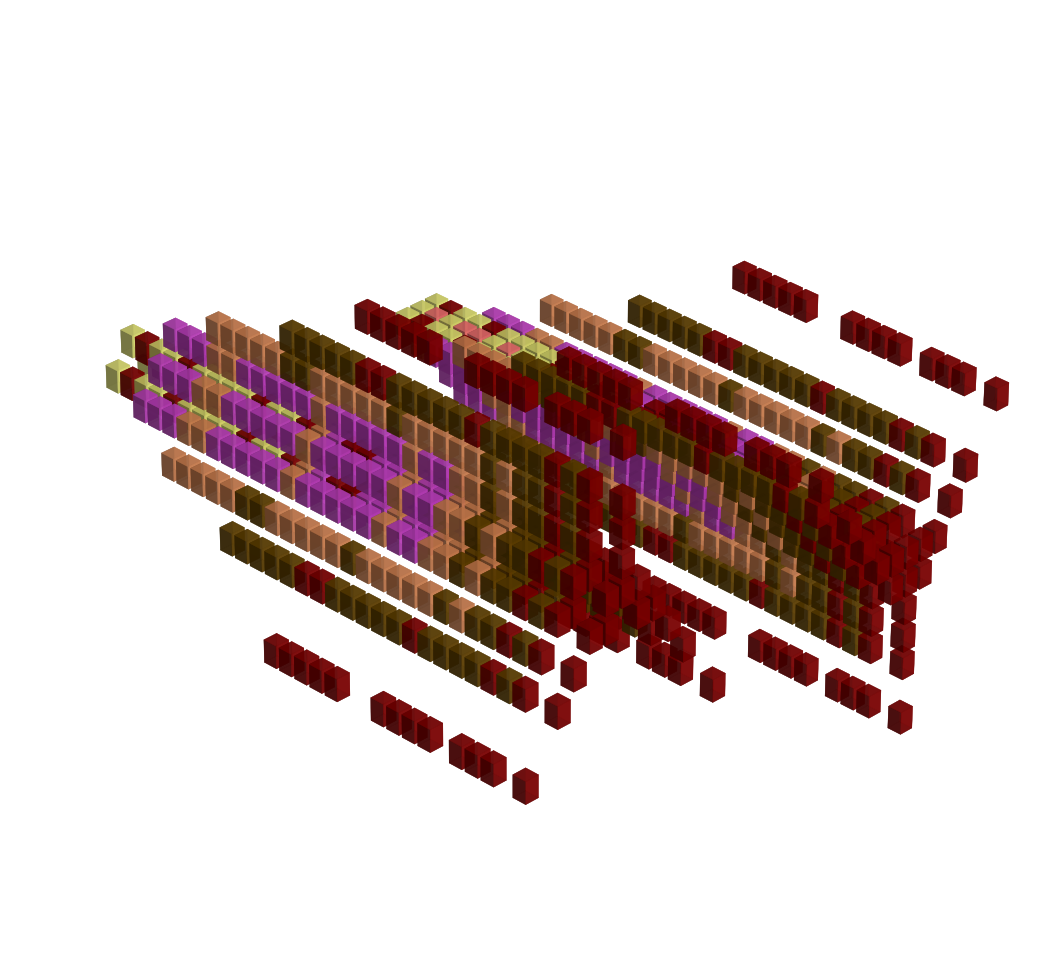
\includegraphics[width=7cm]{src/presets/pattern13-45.png}%           
  \end{adjustbox}                                                        
\caption{Evolution of Preset 13.}                                           
\end{figure}                                                               
                                                                 
                                                                           
\end{minipage}
\hspace{0.1cm}
\begin{minipage}[b]{0.48\linewidth}                                       
\begin{lstlisting}[basicstyle=\ttfamily\scriptsize,caption=Data structure for Preset 13.]
preset13
  .BYTE $00 ; unusedPresetByte
  .BYTE $0B ; smoothingDelay
  .BYTE $01 ; cursorSpeed
  .BYTE $1C ; bufferLength
  .BYTE $02 ; pulseSpeed
  .BYTE $0A ; indexForColorBarDisplay
  .BYTE $07 ; lineWidth
  .BYTE $09 ; sequencerSpeed
  .BYTE $01 ; pulseWidth
  .BYTE $07 ; baseLevel
  ; presetColorValuesArray: 
  .BYTE BLACK,YELLOW,CYAN,LTBLUE,BLUE,RED,PURPLE,LTRED
  .BYTE $00 ; trackingActivated
  .BYTE $00 ; lineModeActivated
  .BYTE $03 ; presetIndex
  .BYTE $03 ; currentPatternElement
  .BYTE $04 ; currentSymmetrySetting
\end{lstlisting}
\end{minipage}

\begin{minipage}[b]{0.48\linewidth}


                                                                 
\begin{figure}[H]                                                          
  \centering                                                             
  \begin{adjustbox}{width=7cm,center}                                   
  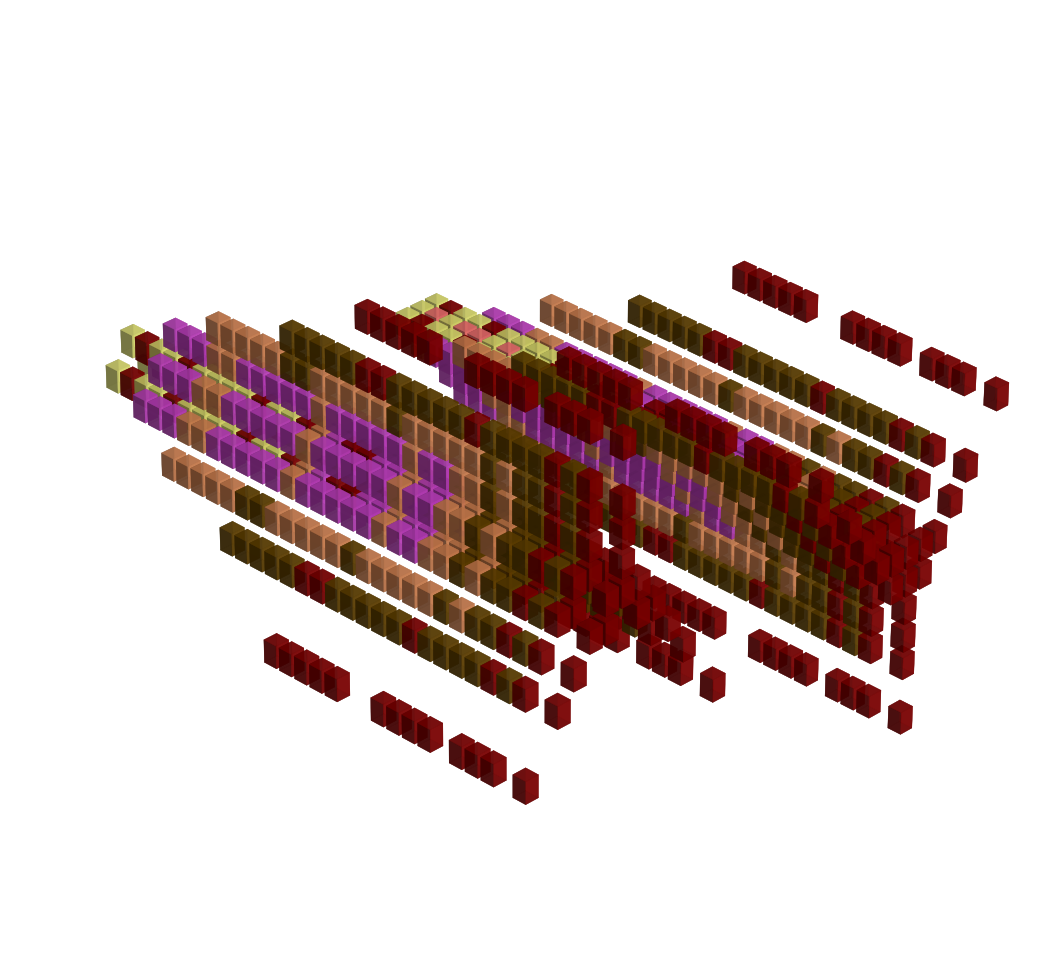
\includegraphics[width=7cm]{src/presets/pattern14-45.png}%           
  \end{adjustbox}                                                        
\caption{Evolution of Preset 14.}                                           
\end{figure}                                                               
                                                                 
                                                                           
\end{minipage}
\hspace{0.1cm}
\begin{minipage}[b]{0.48\linewidth}                                       
\begin{lstlisting}[basicstyle=\ttfamily\scriptsize,caption=Data structure for Preset 14.]
preset14
  .BYTE $00 ; unusedPresetByte
  .BYTE $0C ; smoothingDelay
  .BYTE $02 ; cursorSpeed
  .BYTE $2B ; bufferLength
  .BYTE $01 ; pulseSpeed
  .BYTE $0A ; indexForColorBarDisplay
  .BYTE $07 ; lineWidth
  .BYTE $08 ; sequencerSpeed
  .BYTE $01 ; pulseWidth
  .BYTE $07 ; baseLevel
  ; presetColorValuesArray: 
  .BYTE BLACK,RED,BROWN,ORANGE,PURPLE,RED,YELLOW,LTRED
  .BYTE $FF ; trackingActivated
  .BYTE $00 ; lineModeActivated
  .BYTE $04 ; presetIndex
  .BYTE $04 ; currentPatternElement
  .BYTE $02 ; currentSymmetrySetting
\end{lstlisting}
\end{minipage}

\clearpage
\begin{minipage}[b]{0.48\linewidth}
\begin{figure}[H]                                                          
  \centering                                                             
  \begin{adjustbox}{width=7cm,center}                                   
  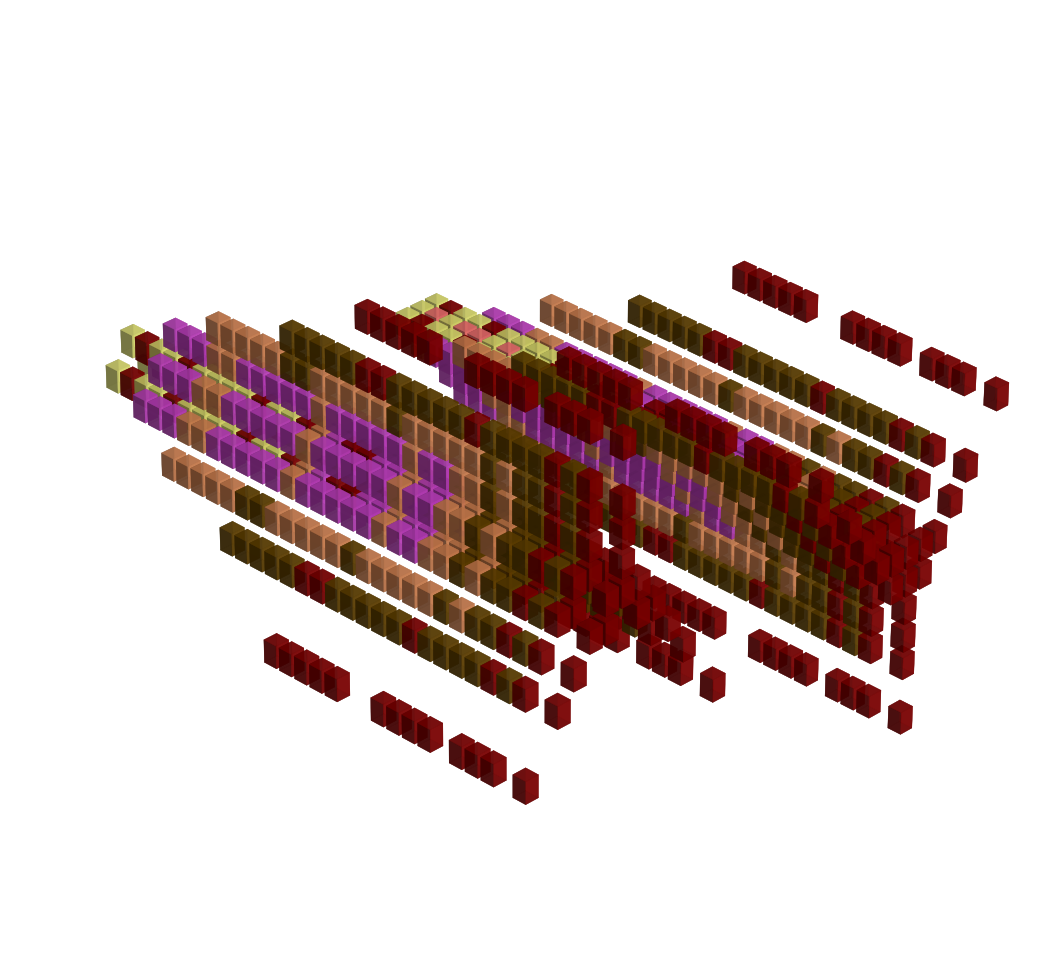
\includegraphics[width=7cm]{src/presets/pattern14-45.png}%           
  \end{adjustbox}                                                        
\caption{Evolution of Preset 15.}                                           
\end{figure}                                                               
                                                                 
                                                                           
\end{minipage}
\hspace{0.1cm}
\begin{minipage}[b]{0.48\linewidth}                                       
\begin{lstlisting}[basicstyle=\ttfamily\scriptsize,caption=Data structure for Preset 15.]
preset15
  .BYTE $00 ; unusedPresetByte
  .BYTE $03 ; smoothingDelay
  .BYTE $01 ; cursorSpeed
  .BYTE $1F ; bufferLength
  .BYTE $06 ; pulseSpeed
  .BYTE $01 ; indexForColorBarDisplay
  .BYTE $07 ; lineWidth
  .BYTE $00 ; sequencerSpeed
  .BYTE $01 ; pulseWidth
  .BYTE $07 ; baseLevel
  ; presetColorValuesArray: 
  .BYTE BLACK,BLUE,RED,PURPLE,GREEN,CYAN,YELLOW,WHITE
  .BYTE $FF ; trackingActivated
  .BYTE $00 ; lineModeActivated
  .BYTE $04 ; presetIndex
  .BYTE $04 ; currentPatternElement
  .BYTE $04 ; currentSymmetrySetting
\end{lstlisting}
\end{minipage}


\clearpage
\textbf{Lines 1189-1231. \icode{\textbf{RefreshPresetData}}} 
\begin{lstlisting}[basicstyle=\ttfamily\scriptsize]
;--------------------------------------------
; RefreshPresetData
;--------------------------------------------
RefreshPresetData    
        PLA 
        TAX 
        JSR GetPresetPointersUsingXRegister
        LDY #BUFFER_LENGTH
        LDA (presetSequenceDataLoPtr),Y
        CMP bufferLength
        BEQ b16C6

        JSR ResetCurrentActiveMode
        JMP LoadSelectedPresetSequence
        ; Returns

        ; Check the preset against current data
        ; and reload if different.
b16C6   LDX #$00
        LDY #SEQUENCER_SPEED
b16CA   LDA (presetSequenceDataLoPtr),Y
        CMP presetColorValuesArray,X
        BNE LoadSelectedPresetSequence
        INY 
        INX 
        CPX #$08
        BNE b16CA

        JMP LoadSelectedPresetSequence

;---------------------------------------------
; GetPresetPointersUsingXRegister
;---------------------------------------------
GetPresetPointersUsingXRegister   
        LDA #>presetSequenceData
        STA presetSequenceDataHiPtr
        LDA #<presetSequenceData
        STA presetSequenceDataLoPtr
        TXA 
        BEQ b1712

        ; Skip through the preset data until we get to the position
        ; storing the preset data for the sequence indicated by the X
        ; register.
b1702   LDA presetSequenceDataLoPtr
        CLC 
        ADC #$20
        STA presetSequenceDataLoPtr
        LDA presetSequenceDataHiPtr
        ADC #$00
        STA presetSequenceDataHiPtr
        DEX 
        BNE b1702
b1712   RTS 

\end{lstlisting}
\clearpage

\textbf{Lines 1189-1231. \icode{\textbf{DisplayPresetMessage}}:} 
\clearpage


